%% LyX 2.3.2 created this file.  For more info, see http://www.lyx.org/.
%% Do not edit unless you really know what you are doing.
\documentclass[english]{article}
\usepackage[T1]{fontenc}
\usepackage[latin9]{inputenc}
\usepackage{geometry}
\geometry{verbose,tmargin=2cm,bmargin=2cm,lmargin=2cm,rmargin=2cm}
\usepackage{amsmath}
\usepackage{graphicx}
\usepackage{babel}
\begin{document}
\begin{figure}
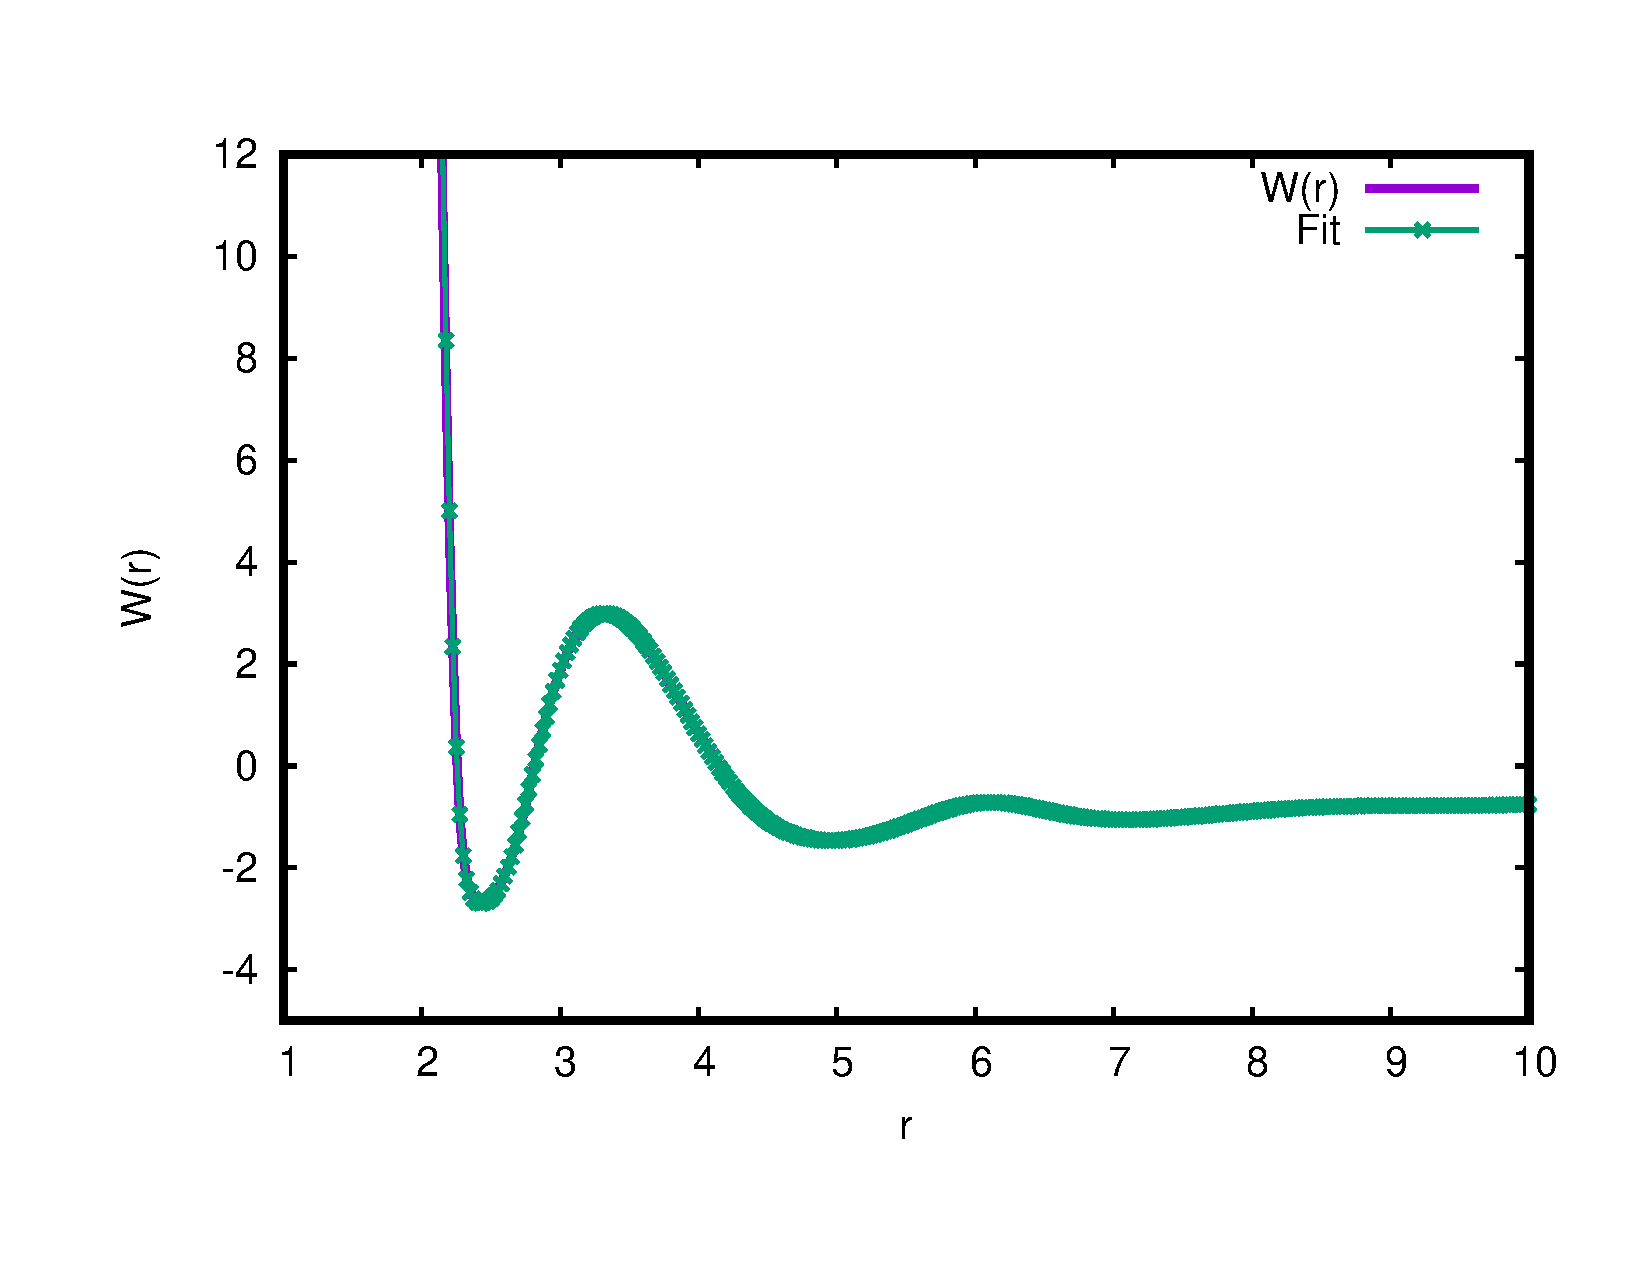
\includegraphics[width=0.5\textwidth]{fit}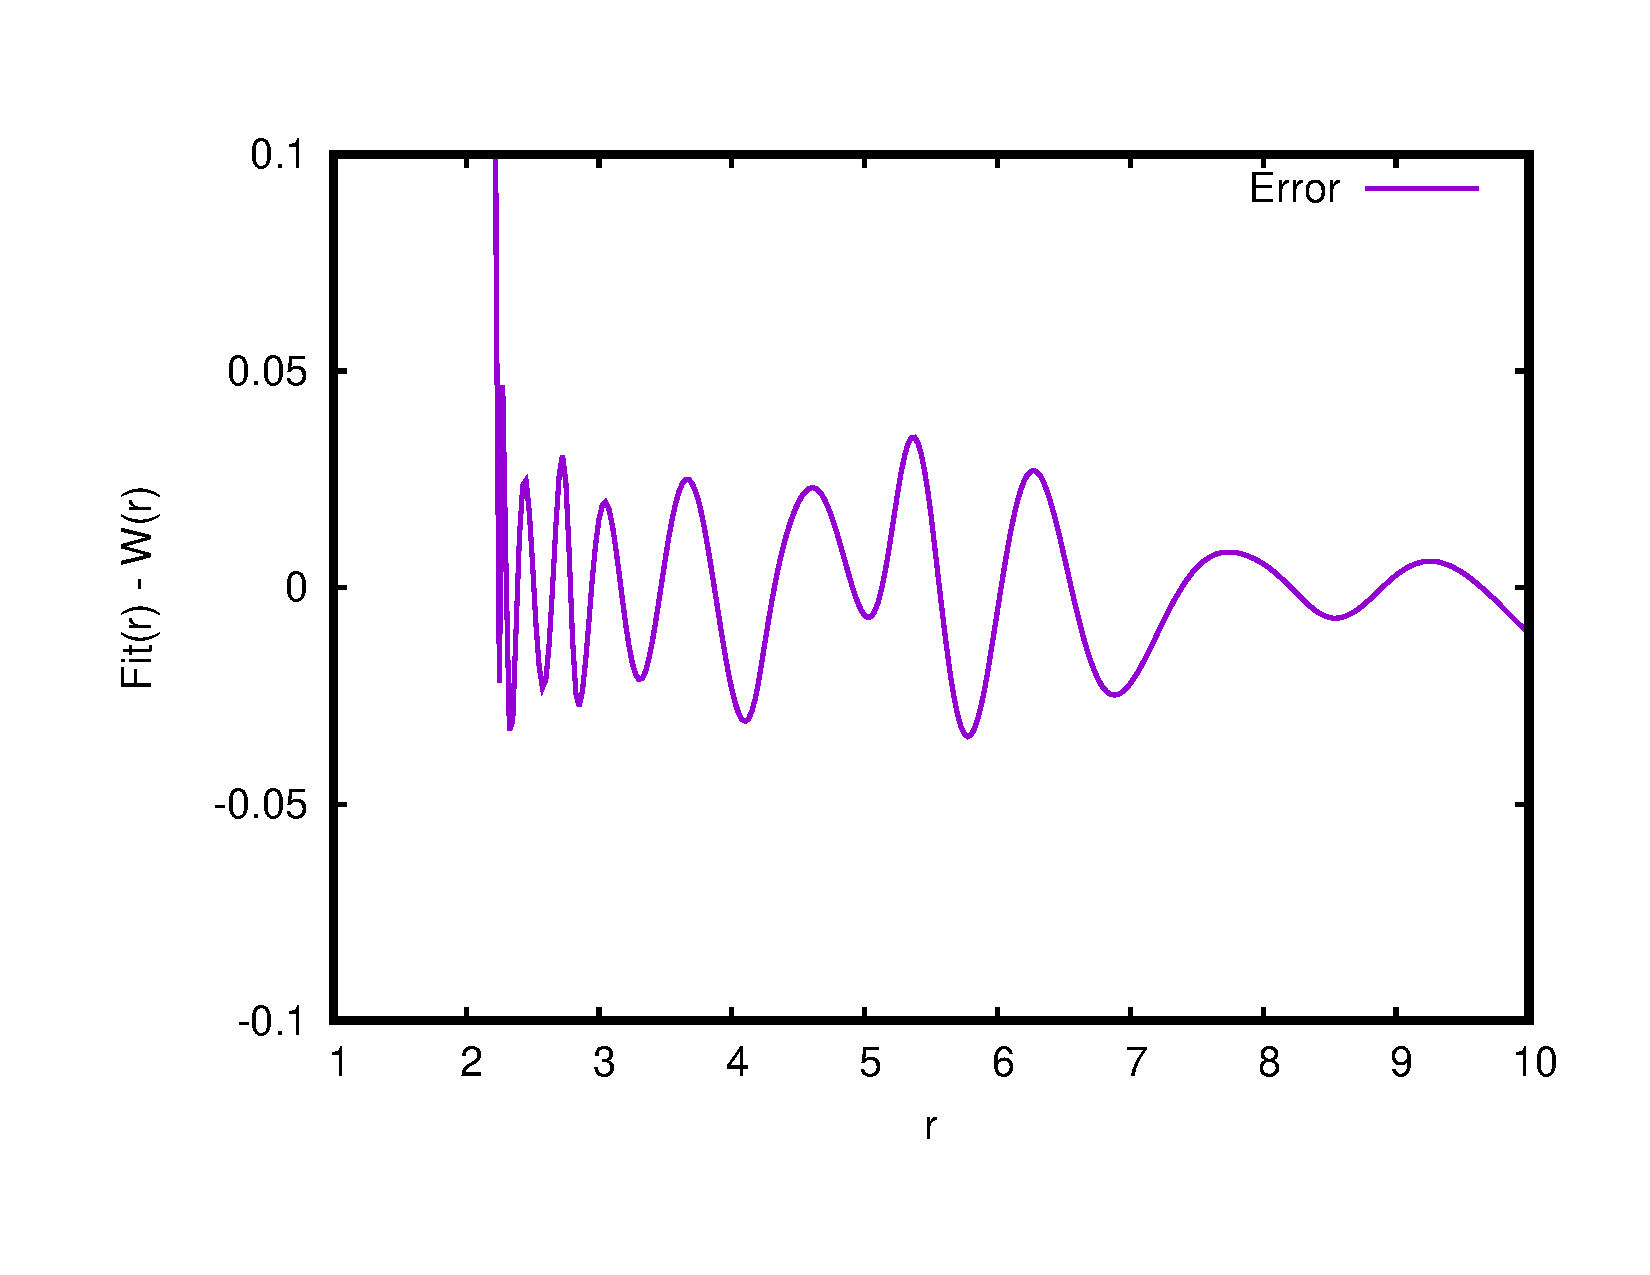
\includegraphics[width=0.5\textwidth]{fit_error}
\end{figure}

\[
W(r)\approx\frac{1}{1+\exp\left(s_{1}(r-s_{2})\right)}\left(\frac{r_{0}}{r}\right)^{\beta}+\sum_{i=1}^{N}a_{i}\exp\left(\frac{-(r-r_{i})^{2}}{w_{i}}\right)-a_{y}\frac{\exp\left(-r_{y}r\right)}{r}
\]

\begin{align*}
N & =4\\
s_{1} & =20.817440\\
s_{2} & =2.218543\\
r_{0} & =2.599721\\
\beta & =15.514784\\
a_{1} & =-2.043783\\
r_{1} & =2.601350\\
w_{i} & =0.095906\\
a_{2} & =5.486850\\
r_{2} & =3.262882\\
w_{2} & =0.749028\\
a_{3} & =0.588646\\
r_{3} & =6.030407\\
w_{3} & =0.418991\\
a_{4} & =0.103249\\
r_{4} & =8.456059\\
w_{4} & =0.786805\\
a_{y} & =8.486511\\
r_{y} & =0.011374
\end{align*}

\end{document}
